\chapter{Overview of the whole Model}

\begin{figure}[H]
\centering
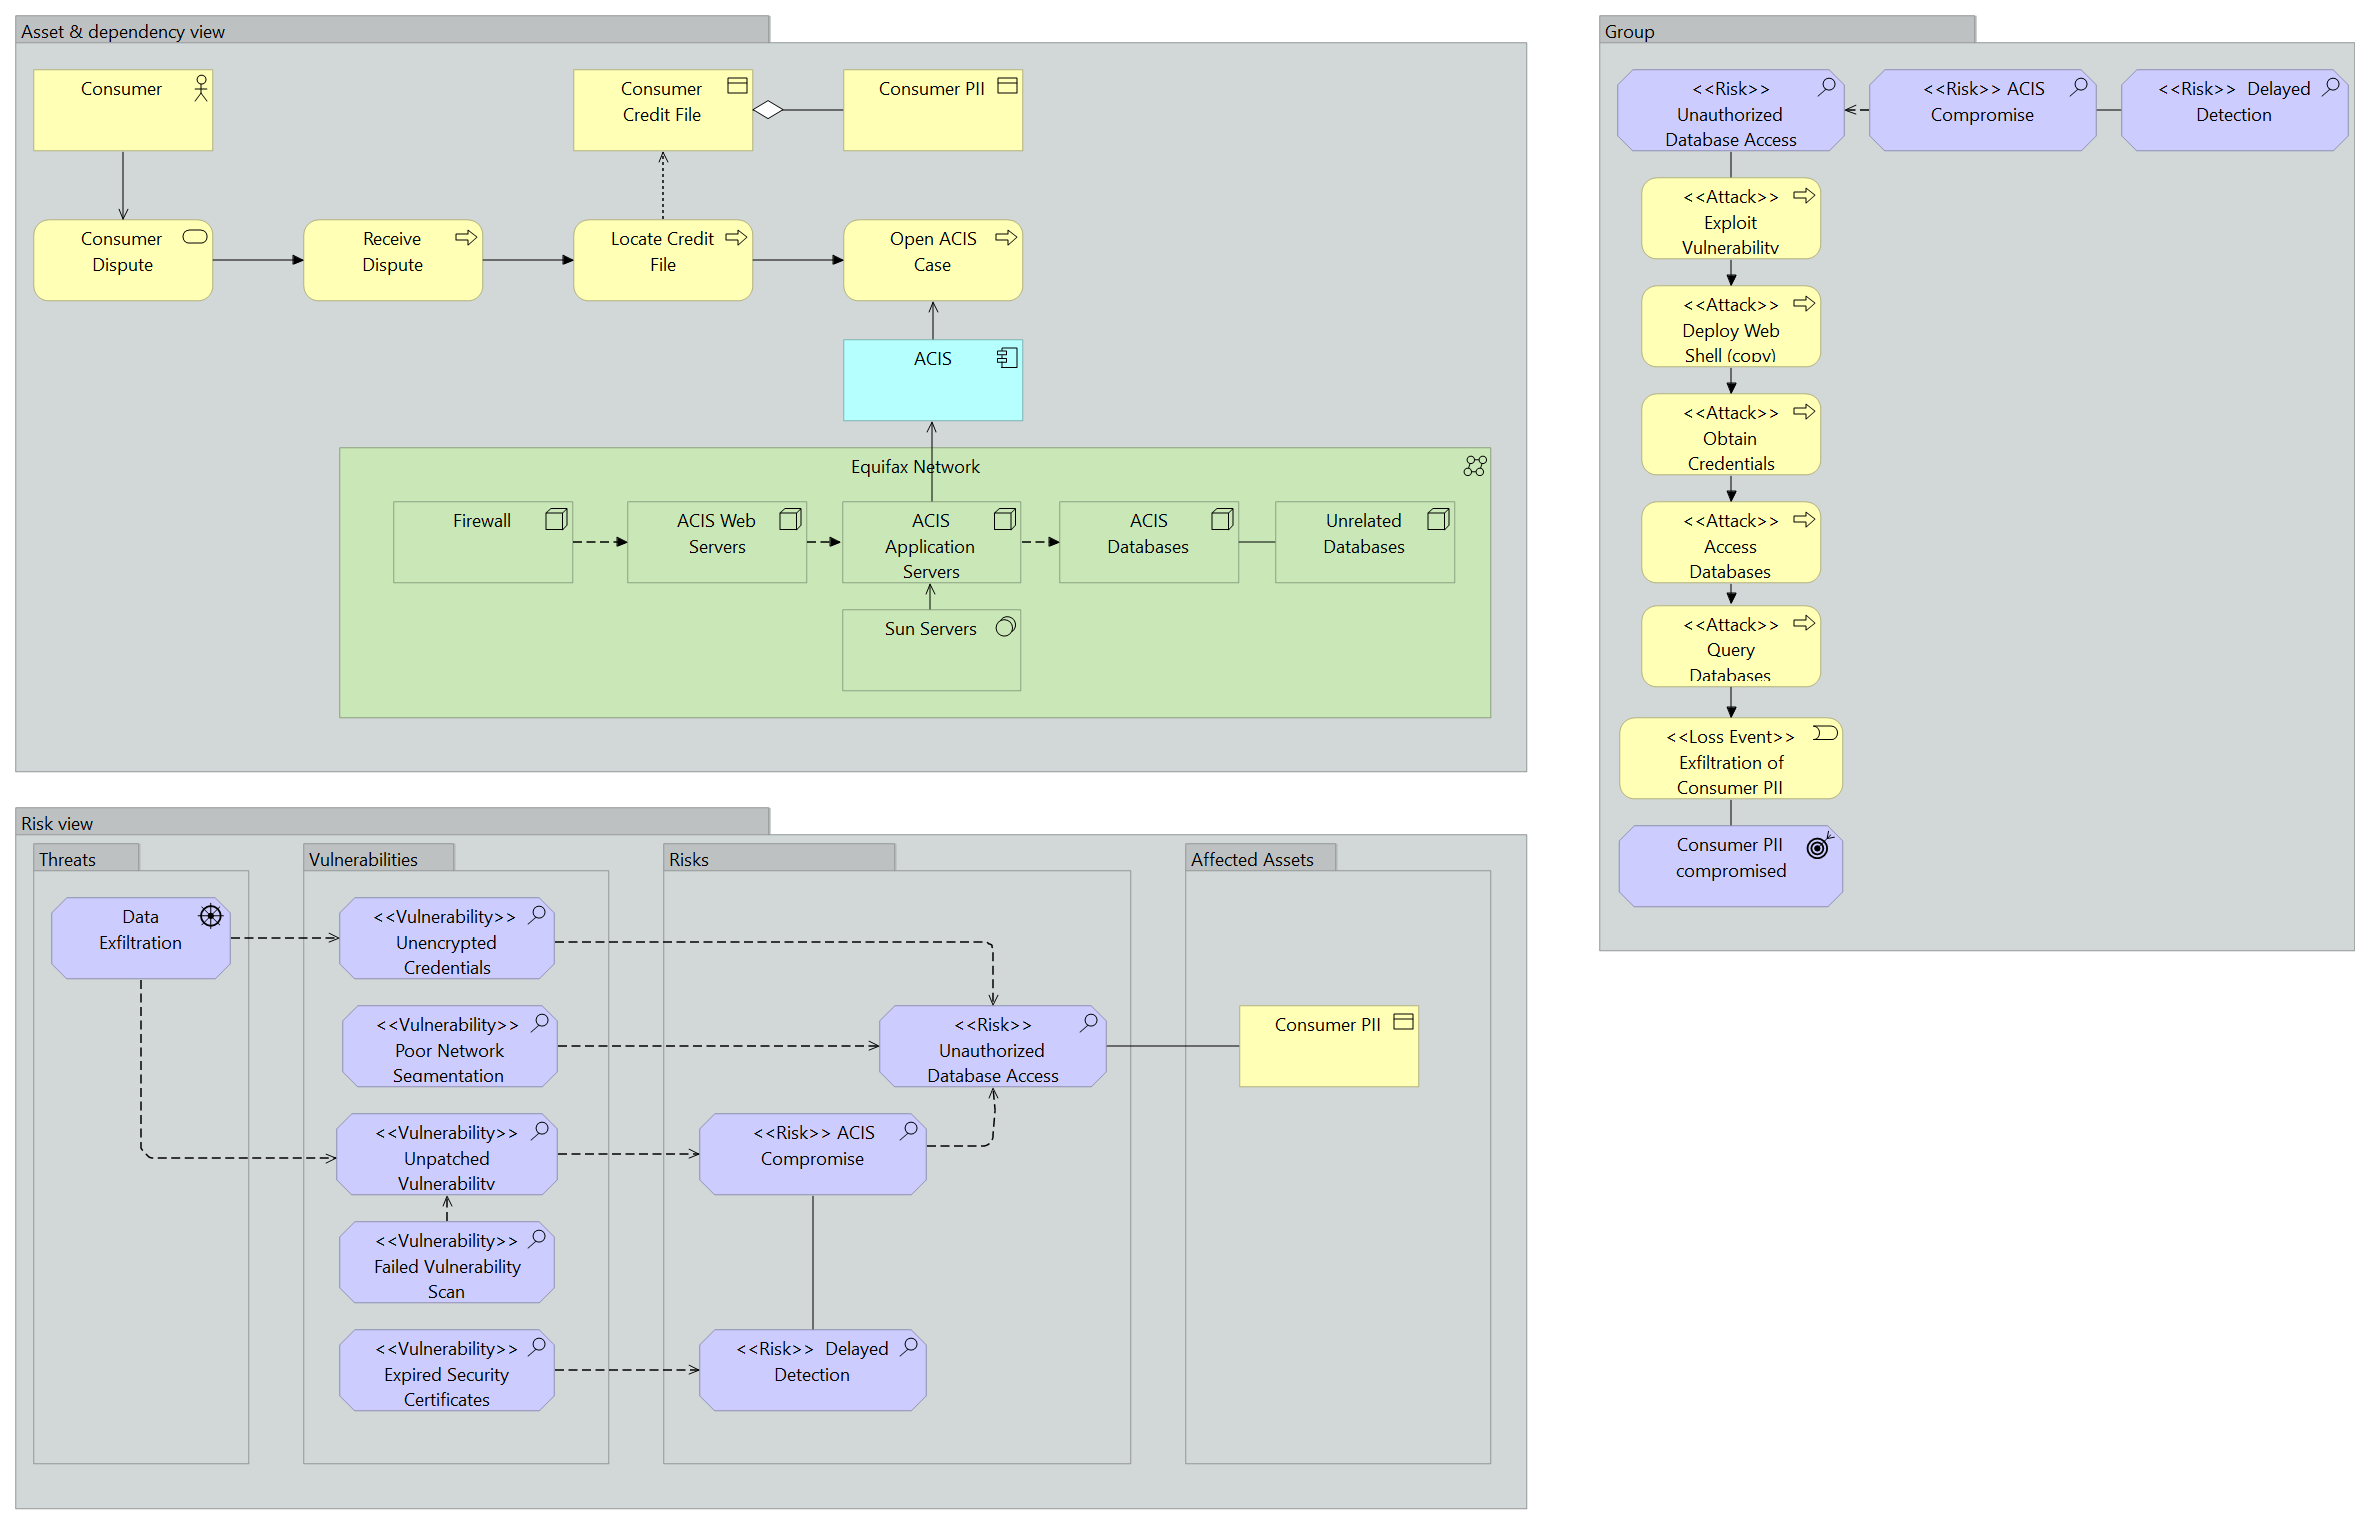
\includegraphics[width=1\linewidth]{images/complete.png}
\caption{Complete view.}
\end{figure}

The complete view of the ArchiMate model combines the business, application, technology and security aspects of the incident. 
\newline
It shows how much a single business process, in this case the consumer dispute process, relies on applications such as ACIS, which in turn heavily relied on it's underlying infrastructure such as it's servers, firewall, databases, etc. in order to function.
\newline
The view also models the dependencies to the security risks identified in the incident, from unencrypted credentials, poor network segmentation to failing detection mechanisms. These vulnerabilities contributed to risks including ACIS compromise, it's delayed detection and unauthorized database access, ultimately affecting consumer's PII.
\newline
Finally, the model shows how the risks turned into an actual attack. The attackers exploited a vulnerability, deployed a web shell, gained credentials, accessed databases, queried them and subsequently exfiltrated consumer's PII.
\newline
Therefore, the complete model connects Equifax's assets and dependencies with the vulnerabilities, risks and attack sequence that resulted in the incident.